\chapter{Implementation}
\label{chap:implementation}

This chapter first justifies the major technology choices
(Section~\ref{sec:impl-technology}), then describes the adaptations to
\texttt{tsm-orchestration} (Section~\ref{sec:impl-tsm}), the data platform
backend and frontend (Sections~\ref{sec:impl-backend} and~\ref{sec:impl-frontend}),
and the unified deployment layer (Section~\ref{sec:impl-deploy}).

%% ----------------------------------------------------------------
\section{Technology Selection}
\label{sec:impl-technology}
%% ----------------------------------------------------------------

The technology choices were driven by the requirements from Chapter~\ref{chap:requirements}
and by maintainability concerns given the expected platform lifetime. Each major choice
is justified below.

\subsection{Backend: FastAPI}
\label{sec:impl-tech-fastapi}

FastAPI~\cite{fastapi-ref} was chosen for the data platform backend. Its
native \texttt{async}/\texttt{await} support enables non-blocking database
queries (via SQLAlchemy~2.0 async sessions) and concurrent HTTP calls to FROST-Server and
GeoServer. Pydantic schemas generate OpenAPI documentation automatically, eliminating the
need to maintain a separate API specification.

\subsection{Frontend: Next.js~15}
\label{sec:impl-tech-nextjs}

Next.js~15~\cite{nextjs-ref} with the App Router was chosen for the frontend portal. React Server
Components render authentication-protected routes on the server, preventing unauthenticated
users from receiving page content. File-based routing and built-in internationalization
support address FR-25 with minimal boilerplate.

\subsection{Time-Series Storage: TimescaleDB}
\label{sec:impl-tech-timescaledb}

TimescaleDB~\cite{timescaledb-ref} was preferred over InfluxDB for time-series storage. As a
PostgreSQL extension, it shares the database server hosting the TSM configuration and
\texttt{water\_dp} schemas, avoiding a separate deployment. Automatic hypertable
chunking, native compression, and full SQL compatibility allow joining observations with
configuration tables directly.

\subsection{Geospatial Layer: GeoServer}
\label{sec:impl-tech-geoserver}

GeoServer~\cite{geoserver-ref} handles geospatial layer management, exposing OGC WMS and WFS
interfaces over PostGIS data. The backend manages workspaces and layers through GeoServer's
REST~API; the frontend renders them with MapLibre~GL.

\subsection{Authentication: Keycloak}
\label{sec:impl-tech-keycloak}

Keycloak~\cite{keycloak-ref} was carried over from the upstream TSM stack. A two-tier RBAC
model splits responsibilities: realm roles define platform-wide privileges, while the
\texttt{project\_members} table stores per-project roles linked through Keycloak groups.
JWT tokens are verified via JWKS endpoint RS256 signatures.

\subsection{Object Storage: MinIO}
\label{sec:impl-tech-minio}

MinIO~\cite{minio-ref} was kept from the upstream stack. Each Thing gets its own bucket;
file uploads trigger the file-ingest worker via S3~event notifications to MQTT. MinIO also
stores user-uploaded parser scripts (Section~\ref{sec:bg-timeio-parsers}).

%% ----------------------------------------------------------------
\section{TSM Orchestration Adaptation}
\label{sec:impl-tsm}
%% ----------------------------------------------------------------

Several targeted adaptations to the upstream \texttt{tsm-orchestration} codebase were required to enable the CZU deployment.
All modifications to upstream files are marked with \texttt{TSM-TEMP-*} identifiers in the codebase to allow clean
identification should a future upstream fix make them redundant. The architectural rationale for these changes
was discussed in Section~\ref{sec:arch-db-staviews}; this section describes their implementation.

\subsection{Local STA Views}
\label{sec:impl-tsm-staviews}

Upstream STA views in \texttt{src/sql/sta\_views/} query tables owned by the external SMS service,
which was non-functional (Section~\ref{sec:bg-timeio-limitations}). The replacement views reside in
\texttt{src/sql/sta\_views\_local/} and query the local \texttt{thing}, \texttt{datastream}, and
\texttt{observation} tables directly.

Nine view files replace the original set, mapping the local \texttt{thing},
\texttt{datastream}, and \texttt{observation} tables to the column layout FROST-Server
expects. Key adaptations include constructing the \texttt{UNIT\_OF\_MEASUREMENT} JSON from
JSONB properties, adding a \texttt{dataSource: local} marker to the observation view output, and deriving
PostGIS geometries from GeoJSON coordinates in Thing properties. Views for
\texttt{SENSORS}, \texttt{FEATURES\_OF\_INTEREST}, and \texttt{OBSERVED\_PROPERTIES}
return empty result sets (\texttt{WHERE false}) so FROST-Server starts without errors.

A corresponding set of Grafana views in \texttt{src/sql/grafana\_views\_local/} provides
a \texttt{datastream\_properties} view used by the Grafana dashboards to display datastream
metadata without depending on SMS tables.

Every file in the local view set begins with a header comment
\texttt{-{}-~TSM-TEMP-DISABLED}, followed by an instruction to revert by deleting the file
and setting \texttt{USE\_LOCAL\_STA\_VIEWS=false}. At runtime, the thing-setup worker checks
this environment variable (defaulting to \texttt{true}) and deploys the local or upstream
view set accordingly during schema provisioning.

\subsection{Compose Modularization}
\label{sec:impl-tsm-compose}

To deploy the data platform alongside TSM without touching the upstream Compose file, a
dedicated overlay was added:
\texttt{docker-compose-water-dp.yml}. This file defines a single service, \texttt{water-dp-api},
that connects to the TSM database, MQTT broker, FROST-Server, and Keycloak instance. The
\texttt{search\_path} is set to \texttt{water\_dp,public} so that the API can access both its own
tables and the TSM configuration tables. The overlay also starts a Redis container for the Celery
task queue.

Because the overlay leaves the upstream \texttt{docker-compose.yml} untouched, it
can be updated independently. The full Compose file chain used by the deployment layer is
described in Section~\ref{sec:impl-deploy-compose}.

\subsection{Worker Architecture}
\label{sec:impl-tsm-workers}

The \texttt{AbstractHandler} base class and its healthcheck mechanism were introduced in
Section~\ref{sec:bg-timeio-workers}. Each worker runs in its own Docker container; scheduling
relies on MQTT topic routing and a cron scheduler. All entrypoints use
\texttt{worker\_launcher.sh}, a Bash wrapper that restarts the process up to three times
within a configurable window before exiting cleanly to prevent infinite restart loops.

Table~\ref{tab:tsm-workers} summarizes each worker's input topic, output, and responsibility.

\begin{landscape}
{\small
\begin{longtable}{p{0.12\linewidth} p{0.20\linewidth} p{0.13\linewidth} p{0.48\linewidth}}
  \caption{TSM worker processes and their MQTT topics.}
  \label{tab:tsm-workers} \\
  \textbf{Worker} & \textbf{Subscribes To} & \textbf{Publishes} & \textbf{Responsibility} \\
  \hline
  \endfirsthead
  \textbf{Worker} & \textbf{Subscribes To} & \textbf{Publishes} & \textbf{Responsibility} \\
  \hline
  \endhead
  configdb-updater
    & \texttt{frontend\_thing\_update}
    & \texttt{configdb\_update}
    & Validates versioned Thing configuration messages (v4--v7) and upserts them into the
      configuration database. \\[4pt]
  thing-setup
    & \texttt{configdb\_update}
    & ---
    & Orchestrates six provisioning sub-handlers: database schema, MinIO bucket, MQTT
      credentials, Grafana dashboard, FROST instance, and crontab entries. \\[4pt]
  mqtt-ingest
    & \texttt{mqtt\_ingest/\#}
    & \texttt{data\_parsed}
    & Parses raw IoT device messages using the parser framework (Section~\ref{sec:impl-tsm-parsers}),
      resolves the Thing by MQTT username, and inserts observations via the database API. \\[4pt]
  file-ingest
    & \texttt{object\_storage\_notification}
    & \texttt{data\_parsed}
    & Parses uploaded CSV or JSON files from MinIO using \texttt{CsvParser} or
      \texttt{JsonParser} and inserts observations. \\[4pt]
  run-qaqc
    & \texttt{data\_parsed}
    & \texttt{qaqc\_done}
    & Runs configurable quality-control tests against newly parsed observations and writes
      quality flags. \\[4pt]
  sync-extapi
    & \texttt{sync\_ext\_apis}
    & \texttt{data\_parsed}
    & Fetches data from external HTTP APIs (e.g.\ DWD weather service) on a cron schedule. \\[4pt]
  sync-extsftp
    & \texttt{sync\_ext\_sftp}
    & ---
    & Downloads files from external SFTP servers into MinIO, which triggers file-ingest
      via S3 event notification. \\[4pt]
  grafana-user
    & \texttt{userinfo\_keycloak}
    & ---
    & Synchronizes Keycloak user accounts with Grafana organizations and roles. \\[4pt]
  monitor-mqtt
    & \texttt{monitor\_mqtt}
    & ---
    & Collects Mosquitto broker metrics (\texttt{\$SYS/broker/}) and writes them to the
      monitoring schema. \\
\end{longtable}
}
\end{landscape}

\subsubsection{Parser Framework}
\label{sec:impl-tsm-parsers}

A class hierarchy rooted in \texttt{AbcParser} forms the parser framework in
\texttt{src/timeio/parser/}. Two branches extend the base: \texttt{PandasParser} for
file-based ingestion (CSV, JSON) and \texttt{MqttParser} for real-time messages with
device-specific subclasses (Campbell~CR6, ChirpStack, DWD API, YDOC~ML-417).

Parsers are resolved at runtime by \texttt{get\_parser()}, which looks up the type string
in a static registry. If no match is found, a dynamic fallback fetches a user-provided
script from MinIO and executes it in an isolated module namespace.

\subsection{Assessment of the TSM-TEMP Approach}
\label{sec:impl-tsm-assessment}

Originally, the \texttt{TSM-TEMP} markers were introduced expecting the upstream SMS to become
operational. At the time of writing, the SMS remains non-functional. The local views fulfil the
same role with lower complexity and a well-defined revert procedure documented in each file's
header comment.

%% ----------------------------------------------------------------
\section{Water Data Platform --- Backend}
\label{sec:impl-backend}
%% ----------------------------------------------------------------


%   - SQLAlchemy 2.0 async ORM patterns
%   - Alembic migration strategy
%
% Key implementation areas:
%   (a) Project-oriented data model: linking sensors to projects across the TSM schema boundary
%   (b) FROST API client: querying and creating Things/Datastreams without direct DB access
%   (c) Alert evaluation: definitions (threshold, comparison, target datastream),
%                          MQTT-triggered worker, alert state machine
%   (d) GeoServer integration via REST API
%   (f) Keycloak OIDC: token validation middleware, per-project role enforcement

Built on FastAPI, the data platform API acts as the application-logic layer on top of
\texttt{tsm-orchestration}. It is structured as a layered Python package in \texttt{api/app/}
with four tiers: endpoint routers, Pydantic\footnote{Pydantic data validation library: \url{https://docs.pydantic.dev/}} schemas, service classes, and SQLAlchemy\footnote{SQLAlchemy ORM: \url{https://www.sqlalchemy.org/}} models.

\subsection{Project Structure}
\label{sec:impl-backend-structure}

Inside \texttt{api/app/}, the code follows a conventional layered layout:

\begin{itemize}
  \item \textbf{Endpoints} (\texttt{api/v1/endpoints/}) --- sixteen router modules, each
        responsible for one REST resource. All routers are assembled into a single
        \texttt{APIRouter} in \texttt{api/v1/api.py} and mounted under the
        \texttt{/api/v1} prefix.
  \item \textbf{Schemas} (\texttt{schemas/}) --- Pydantic v2 models for request validation
        and response serialization. A \texttt{frost/} sub-package provides typed models for
        STA entities (\texttt{Thing}, \texttt{Datastream}, \texttt{Observation}).
  \item \textbf{Services} (\texttt{services/}) --- business-logic classes that the endpoints
        delegate to. A \texttt{timeio/} sub-package encapsulates all integration points with
        the TSM stack: FROST client, MQTT publisher, orchestrator, and direct database access.
  \item \textbf{Models} (\texttt{models/}) --- SQLAlchemy~2.0 ORM classes mapped to the
        \texttt{water\_dp} schema. A shared \texttt{BaseModel} mixin provides audit columns
        (\texttt{created\_at}, \texttt{updated\_at}, \texttt{created\_by},
        \texttt{updated\_by}).
  \item \textbf{Tasks} (\texttt{tasks/}) --- Celery task definitions for asynchronous work:
        alert evaluation, sensor activity recording, inactivity monitoring, and data
        simulation.
  \item \textbf{Worker} (\texttt{worker/}) --- MQTT subscriber that bridges TSM events to
        Celery tasks.
\end{itemize}

In \texttt{main.py}, middleware is applied for request logging, security headers, structured
error responses, CORS, trusted hosts, and rate limiting. OpenAPI documentation is exposed only
in debug mode.

Alembic manages the \texttt{water\_dp} schema evolution through four migration files covering
projects, dashboards, geospatial layers, alerts, RBAC, and sensor activity tracking.

\subsection{Project and Sensor Management}
\label{sec:impl-backend-projects}

At the core of the data model is the \emph{project}, grouping sensors, alerts, dashboards, and
members into a logical unit. The \texttt{Project} model stores metadata (name, description,
visibility) and references a Keycloak group through \texttt{authorization\_provider\_group\_name}.
Sensors are linked to projects via the \texttt{project\_sensors} association table, which maps
a project UUID to a Thing UUID in the TSM configuration database.

Project CRUD, member management, and sensor-project
associations are handled by the \texttt{ProjectService}. When a sensor is linked to a project, the service resolves the Thing's schema
name through the TSM configuration database, enabling the API to query observations in the
correct per-thing schema. Core sensor operations are provided by \texttt{AsyncThingService}
through the asynchronous FROST client: listing Things, fetching Datastreams, and retrieving
time-filtered Observations. A synchronous \texttt{ThingService} variant exists for use in
Celery tasks, where an async event loop is not available.

Sensor creation follows the Thing lifecycle described in Section~\ref{sec:arch-mqtt-lifecycle}.
Located in \texttt{services/timeio/orchestrator.py}, the \texttt{TimeIOOrchestrator} constructs the
configuration payload, derives the schema name from the Keycloak group, generates MQTT and
S3 credentials, and publishes the message to \texttt{frontend\_thing\_update}. Downstream
TSM workers then provision the infrastructure automatically.

\subsection{FROST API Client Integration}
\label{sec:impl-backend-frost}

Two FROST client variants exist: a synchronous one (\texttt{requests}) and an asynchronous
one (\texttt{httpx}), both exposing the same interface for Thing, Datastream, Observation,
and Location retrieval with STA pagination. URL routing follows the FROST multi-tenancy
pattern \texttt{\{base\_url\}/\{project\_name\}/\{version\}/\{path\}}. The
asynchronous variant is used for concurrent operations (e.g.\ fetching Things across
projects); the synchronous variant serves Celery tasks where no event loop is available.

\subsection{Alert Evaluation System}
\label{sec:impl-backend-alerts}

Three components form the alert system: definitions, evaluators, and a state machine. An
\texttt{AlertDefinition} is created per project and specifies: the target (a specific
datastream or a QA/QC rule), conditions (field, operator, threshold), and an active flag.

Two evaluation entry points are exposed by \texttt{AlertEvaluator}:

\begin{enumerate}
  \item \textbf{Sensor data evaluation} --- \texttt{evaluate\_all\_active\_sensor\_rules()}
        periodically queries the latest observation for each targeted datastream and
        evaluates threshold conditions. Conditions specify an operator (\texttt{>},
        \texttt{<}, \texttt{==}) and a threshold value.
  \item \textbf{QA/QC evaluation} --- \texttt{evaluate\_qaqc\_rules\_for\_thing()} queries
        the per-thing observation table directly via \texttt{psycopg2}, computes the ratio
        of flagged observations within a configurable time window, and compares against
        the threshold. Flag levels are classified as \texttt{BAD} (quality value $\geq 255$),
        \texttt{QUESTIONABLE} ($\geq 2$), or \texttt{ANY} ($> 0$).
\end{enumerate}

MQTT integration (Section~\ref{sec:arch-mqtt-alerts}) bridges TSM events to the
evaluator: the \texttt{mqtt\_handler.py} subscriber receives \texttt{qaqc\_done} messages
and dispatches the \texttt{evaluate\_qaqc\_alerts\_for\_thing} Celery task with the
affected Thing's UUID. Similarly, \texttt{data\_parsed} messages trigger the
\texttt{record\_sensor\_activity} task for inactivity monitoring.

Alert deduplication is enforced by checking for existing active alerts per definition before
creating new ones. The three-state lifecycle and automatic resolution logic are described
in Section~\ref{sec:arch-mqtt-alerts}.

\subsection{GeoServer Integration}
\label{sec:impl-backend-geoserver}

In \texttt{services/geoserver\_service.py}, the \texttt{GeoServerService} wraps the GeoServer
REST~API for programmatic layer management. All operations use HTTP Basic authentication
against the GeoServer admin account.

Available operations include workspace creation, PostGIS datastore configuration, and
layer publishing. The \texttt{publish\_layer()} method registers a new feature type with a
specified spatial reference system (SRS), default style, and visibility. The
\texttt{publish\_sql\_view()} method creates layers backed by parameterized SQL views using
GeoServer's \texttt{JDBC\_VIRTUAL\_TABLE} metadata, which enables dynamic per-project
sensor views without pre-creating database views.

Geospatial features are stored in the \texttt{water\_dp} schema using GeoAlchemy2\footnote{GeoAlchemy2 spatial extension for SQLAlchemy: \url{https://geoalchemy-2.readthedocs.io/}}
\texttt{Geometry} columns (SRID~4326). The \texttt{GeoLayer} and \texttt{GeoFeature} models
represent uploaded layers and their individual features. Layer-to-project associations
are managed through the \texttt{LayerProjectAssignment} model.

\subsection{Authentication and Authorization}
\label{sec:impl-backend-auth}

Token validation is implemented in \texttt{core/security.py}. It fetches the JWKS
from Keycloak's well-known endpoint and verifies RS256 signatures on incoming JWT tokens.
JWKS data is cached with a one-hour TTL and refreshed under an \texttt{asyncio.Lock} to
prevent concurrent refresh requests. Multi-issuer support allows tokens issued by the
internal Keycloak URL, the Docker-internal address (\texttt{keycloak:8080}), and an optional
external URL to be accepted.

Three levels of access control are provided by the dependency chain in \texttt{api/deps.py}: \texttt{get\_current\_user()} extracts and verifies the bearer token,
\texttt{has\_role()} checks for a specific Keycloak realm role, and
\texttt{get\_current\_active\_superuser()} verifies administrator privileges.

Per-project authorization uses the two-tier RBAC model described in
Section~\ref{sec:impl-tech-keycloak}. The \texttt{RBACService} in
\texttt{services/rbac\_service.py} resolves the effective role by evaluating six rules in
priority order:
\begin{enumerate}
  \item Realm administrator receives owner access to all projects.
  \item Keycloak group administrator receives owner access to projects in their group.
  \item An explicit \texttt{project\_members} row grants the stored role.
  \item The original project creator is treated as owner for backward compatibility.
  \item Any member of the project's Keycloak group is granted viewer access.
  \item If none of the above match, the request is rejected with HTTP~403.
\end{enumerate}
The JWT \texttt{groups} claim is parsed by
\texttt{parse\_group\_roles()}, which extracts the Keycloak subgroup suffix
(e.g.\ \texttt{/GroupName/editors} yields role \texttt{editor}). The resolved role determines
the capability set: \texttt{can\_view}, \texttt{can\_edit\_settings},
\texttt{can\_edit\_alerts}, \texttt{can\_link\_sensors}, \texttt{can\_manage\_members},
\texttt{can\_delete}, \texttt{global\_sms\_access}, and \texttt{global\_layers\_access}.

%% ----------------------------------------------------------------
\section{Water Data Platform --- Frontend Portal}
\label{sec:impl-frontend}
%% ----------------------------------------------------------------

Built on Next.js~15 with React\footnote{React UI library: \url{https://react.dev/}}~19, the frontend portal uses the App~Router architecture. The
application is deployed under the \texttt{/portal} base path and built in \texttt{standalone}
output mode for containerized deployment.

\subsection{Information Architecture}
\label{sec:impl-frontend-ia}

Routing follows the App~Router convention, where each directory under
\texttt{app/} corresponds to a URL segment. The major route groups are:

\begin{itemize}
  \item \textbf{\texttt{/projects}} --- project list, creation, and per-project views. Each
        project page (\texttt{/projects/[id]}) provides sub-routes for sensor data
        (\texttt{/data}), individual sensor time-series (\texttt{/data/[sensorId]}),
        dashboards (\texttt{/dashboards}), alerts, QA/QC configuration, sensor simulator,
        and project settings.
  \item \textbf{\texttt{/sms}} --- Sensor Management System interface for sensor, parser,
        device type, and external API type administration. Access is restricted to users
        with at least the \texttt{editor} role.
  \item \textbf{\texttt{/layers}} --- GeoServer layer management: listing, upload, and
        detail views.
  \item \textbf{\texttt{/settings}} --- user profile and password management.
\end{itemize}

All authenticated routes use a protected layout pattern. Each layout calls the server-side
\texttt{auth()} function from NextAuth and redirects unauthenticated users to the sign-in
page. The SMS and Layers layouts additionally check the JWT group role to enforce the minimum
\texttt{editor} privilege. At the top level, the root layout wraps the entire application in a \texttt{Providers}
component that supplies the React~Query\footnote{TanStack Query (React Query): \url{https://tanstack.com/query}} \texttt{QueryClientProvider}, the NextAuth\footnote{NextAuth.js authentication library: \url{https://next-auth.js.org/}}
\texttt{SessionProvider}, a theme context, and an idle-timeout monitor.

Figure~\ref{fig:screenshot-project-list} shows the project list, which serves as
the main landing page after login. Projects are displayed as cards with their
description and linked sensor count; a group filter allows narrowing the view
by Keycloak group membership.

\begin{figure}[ht]
  \centering
  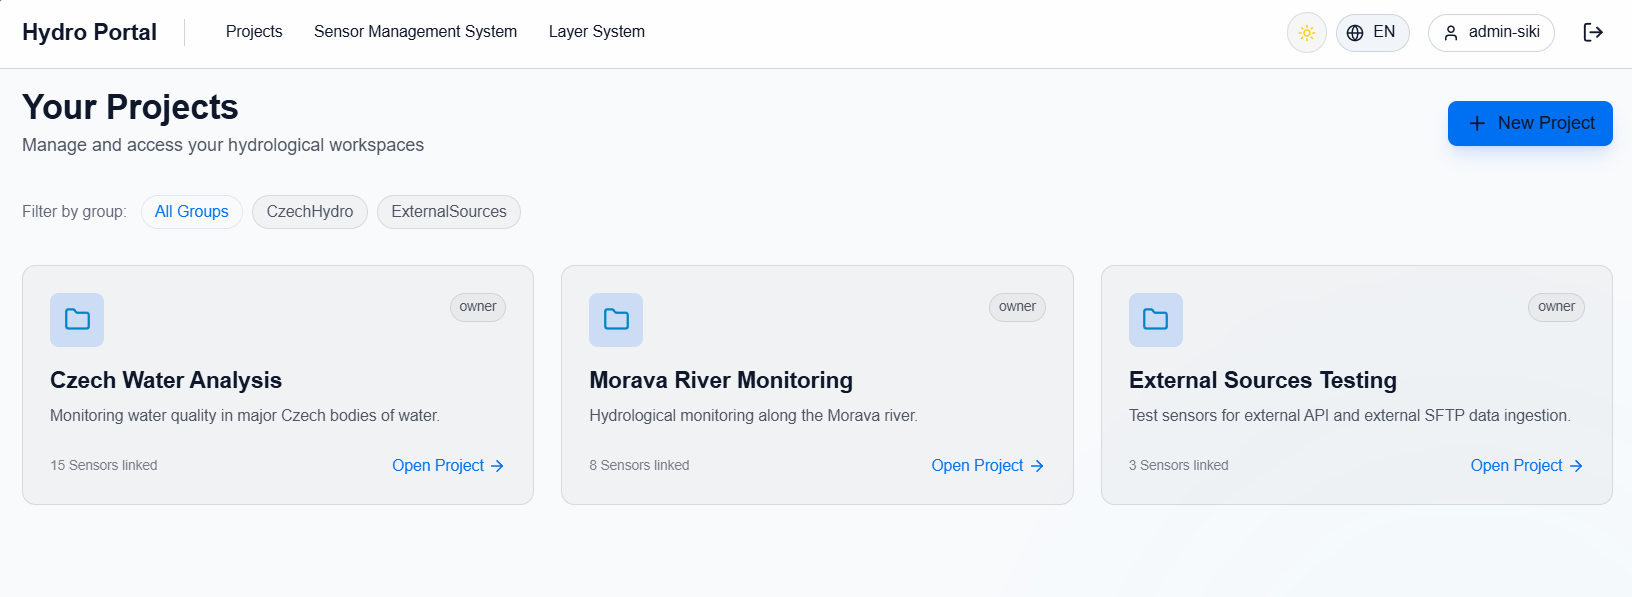
\includegraphics[width=0.95\textwidth]{figures/screenshot-dashboard.png}
  \caption{Project list page. Each card shows the project name, description,
           number of linked sensors, and the user's role. The group filter
           at the top restricts the view to a single Keycloak group.}
  \label{fig:screenshot-project-list}
\end{figure}

\subsection{Time-Series Visualization}
\label{sec:impl-frontend-charts}

Multi-series time-series data is rendered by the \texttt{TimeSeriesChart} component using the
Recharts\footnote{Recharts charting library: \url{https://recharts.org/}} library. Interactive zoom is supported via two mechanisms: a
\texttt{ReferenceArea} drawn by click-and-drag to select a time range, and a
\texttt{Brush} component for scrolling through the full dataset. Multiple series
(each with its own color, label, and unit) are merged into a unified time axis by indexing
all data points into a shared timestamp map.

Data is fetched through React~Query hooks in \texttt{hooks/queries/}, which provide
caching, background refetching, and loading-state management. Ten query-hook modules
cover the major resource types: projects, sensors, dashboards, alerts, QA/QC,
SMS, layers, simulator, and permissions. Query keys are centralized in
\texttt{hooks/queries/keys.ts} to ensure cache consistency across components.

An Axios\footnote{Axios HTTP client: \url{https://axios-http.com/}} instance in \texttt{lib/api.ts} serves as the API client, with a request interceptor that
attaches the NextAuth access token as a \texttt{Bearer} header. An in-memory token cache
with a 60-second expiry buffer avoids redundant \texttt{getSession()} calls.

Figure~\ref{fig:screenshot-sensor-detail} shows the per-project sensor detail
view for the Orl\'{\i}k Dam monitoring station. The left panel displays metadata
(status, device type, description, coordinates) and a location mini-map; the
right panel renders a time-series chart of recent observations with a datastream
selector.

\begin{figure}[ht]
  \centering
  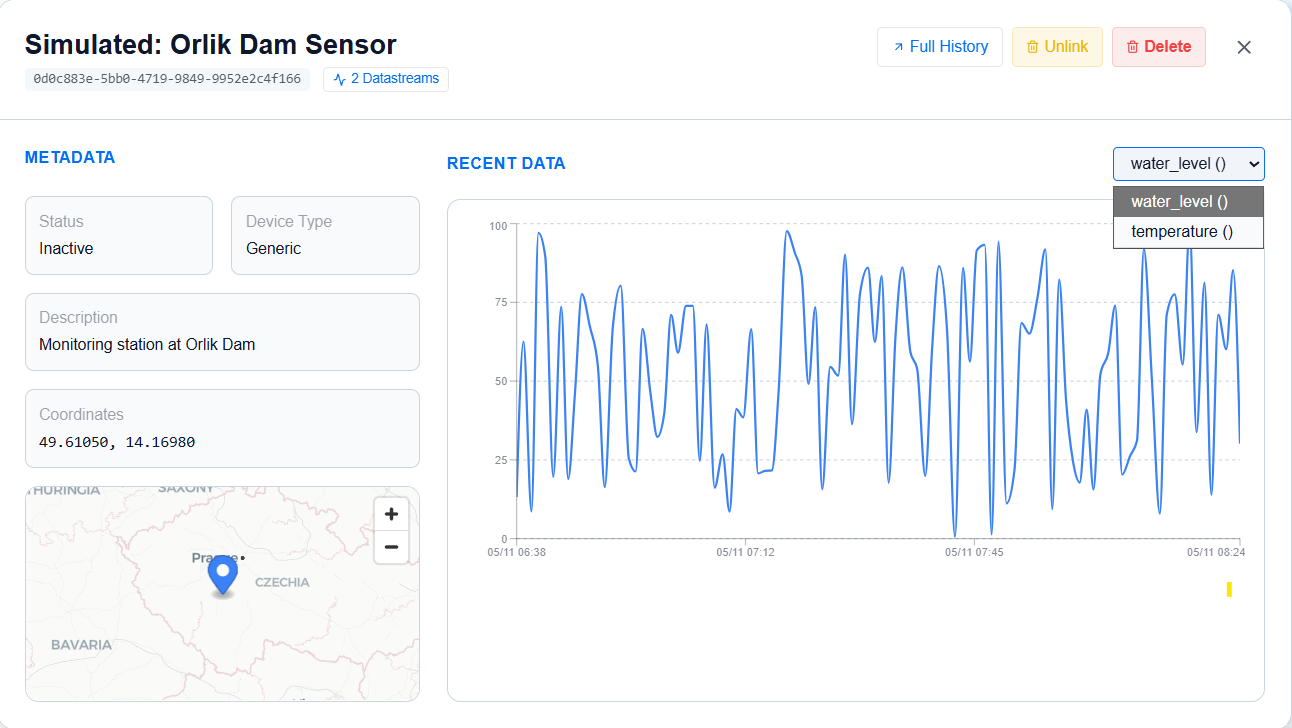
\includegraphics[width=0.95\textwidth]{figures/screenshot-timeseries.png}
  \caption{Sensor detail view within a project. The metadata panel on the left
           shows the sensor status, device type, coordinates, and a location
           mini-map. The chart on the right plots recent observations for the
           selected datastream (\texttt{water\_level}); a dropdown allows
           switching between available datastreams.}
  \label{fig:screenshot-sensor-detail}
\end{figure}

\subsection{Geospatial Layer Viewer}
\label{sec:impl-frontend-geo}

Geospatial rendering uses MapLibre~GL~JS\footnote{MapLibre GL JS mapping library: \url{https://maplibre.org/}} in three components. Sensor locations appear as clustered GeoJSON markers on a CARTO basemap
in the \texttt{ProjectMap} component
(dark-matter or positron, selected by the theme context). Marker popups show the latest
datastream values, refreshed every 30~seconds. GeoServer WMS layers assigned to the
project are overlaid as raster tiles, and a layer-switching menu allows users to
toggle their visibility.

An interactive click-or-drag marker in the \texttt{LocationPickerMap} component enables
setting sensor coordinates during Thing creation. A read-only map in \texttt{SensorMiniMap} shows the sensor's location.

Figure~\ref{fig:screenshot-map} illustrates the map view with a GeoServer WMS
layer overlay (Czech Republic boundaries) and sensor markers distributed across
the monitored region.

\begin{figure}[ht]
  \centering
  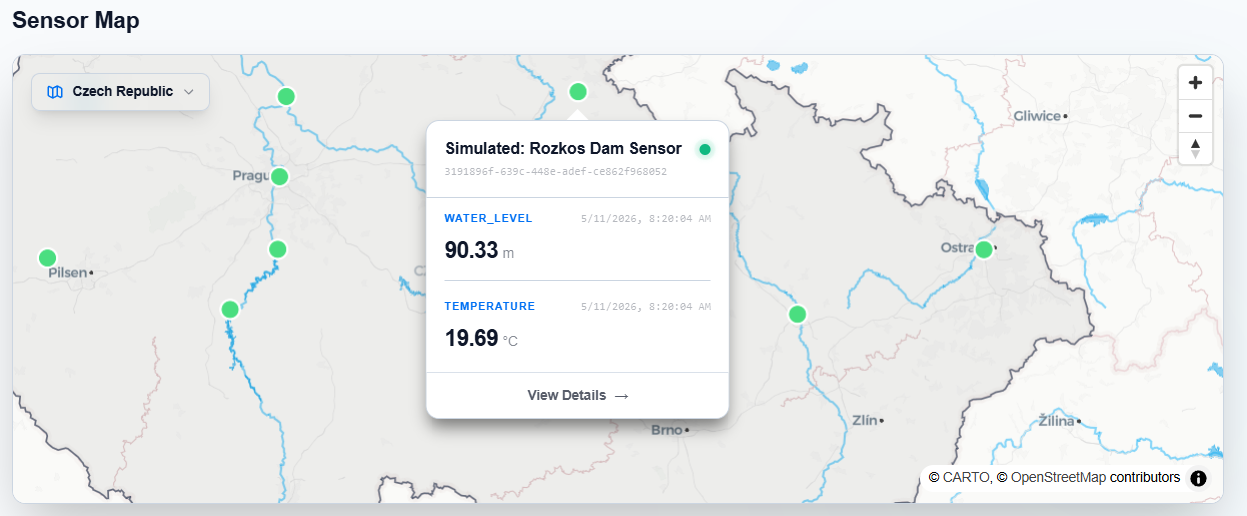
\includegraphics[width=0.95\textwidth]{figures/screenshot-map.png}
  \caption{Sensor map on a CARTO positron basemap with a GeoServer WMS layer
           overlay. The popup for the Rozko\v{s} Dam sensor shows the latest
           \texttt{water\_level} (90.33\,m) and \texttt{temperature}
           (19.69\,\textdegree{}C) readings. A layer selector in the top-left
           corner toggles WMS overlays.}
  \label{fig:screenshot-map}
\end{figure}

\subsection{Data Quality Interface}
\label{sec:impl-frontend-quality}

Accessible at two levels, per-project (\texttt{/projects/[id]/qaqc})
and globally through the SMS section (\texttt{/sms/qa-qc}), the QA/QC interface. The \texttt{SensorQAQCSection}
component renders the QC test configuration for a single sensor, allowing users to define
test types, thresholds, and parameters. A dedicated API client (\texttt{lib/qaqc-api.ts})
provides typed functions for three endpoint scopes: SMS-level, Thing-level, and
project-level QA/QC configuration.

\subsection{Batch Import}
\label{sec:impl-frontend-batch}

A drag-and-drop CSV upload workflow is provided by the \texttt{BulkImportDialog} component for
creating multiple sensors in a single operation. The \texttt{DataUploadModal} and
\texttt{DatasetUploadModal} components handle historical observation data import: users
upload CSV files which are stored in the per-Thing MinIO bucket, triggering the TSM
file-ingest pipeline. The per-sensor data view also includes a \texttt{FileUploadDialog}
for individual file uploads.

\subsection{Multilingual Support}
\label{sec:impl-frontend-i18n}

Three languages are supported by the portal: English, Czech, and Slovak. A custom solution based on a Zustand\footnote{Zustand state management library: \url{https://github.com/pmndrs/zustand}} store (\texttt{useLanguageStore}) with
\texttt{persist} middleware, which saves the selected language to \texttt{localStorage}
under the key \texttt{language-storage}. Locale files in \texttt{locales/} export typed
\texttt{Dictionary} objects (\texttt{en.ts}, \texttt{cs.ts}, \texttt{sk.ts}) that share
a common interface definition.

The \texttt{useTranslation()} hook returns a \texttt{t(path, params?)} function that
traverses the dictionary by dot-notation keys (e.g.\ \texttt{t('header.projects')}) and
supports \texttt{\{\{param\}\}} interpolation. In the application header, a \texttt{LanguageSwitcher} component allows users to switch the language at runtime.

Locale selection is purely client-side; there is no server-side locale detection or
URL-based language routing. This design was chosen to simplify the deployment and avoid
additional Next.js middleware complexity, at the cost of the initial page flash before
the persisted language is loaded from storage.

Figure~\ref{fig:screenshot-sms} shows the Sensor Management System interface, which
is accessible only to users with the \texttt{editor} role or higher.

\begin{figure}[ht]
  \centering
  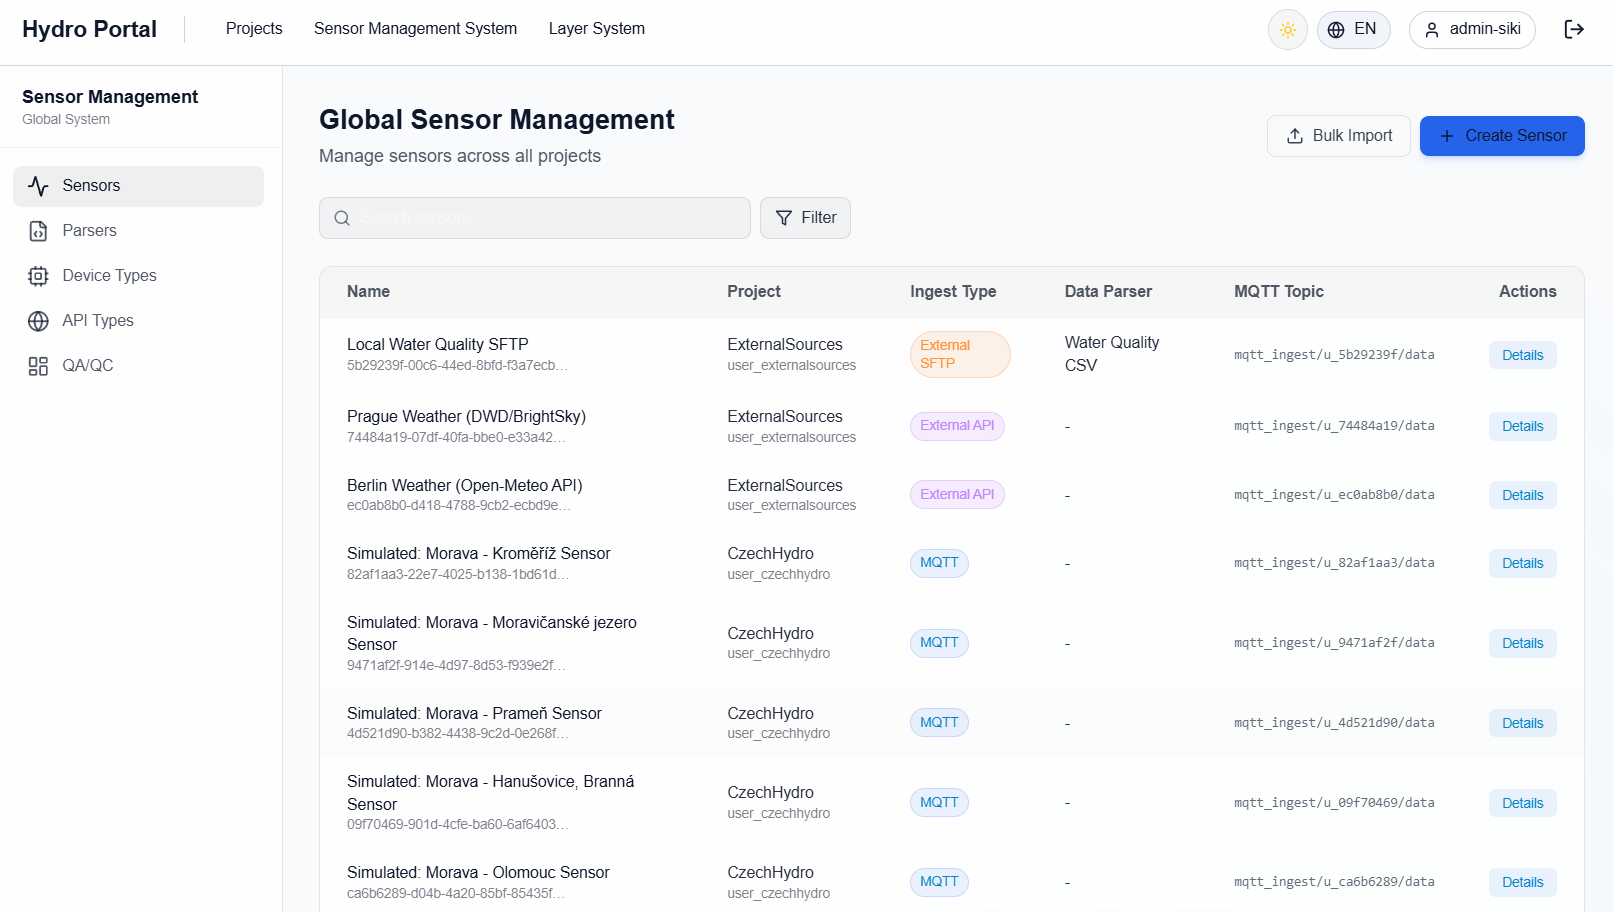
\includegraphics[width=0.95\textwidth]{figures/screenshot-sms.png}
  \caption{Global Sensor Management page in the SMS section. Each row shows
           the sensor name, owning project, ingestion type (MQTT, External~API,
           or External~SFTP), assigned data parser, and the MQTT topic. The
           sidebar provides navigation to parsers, device types, API types,
           and QA/QC configuration.}
  \label{fig:screenshot-sms}
\end{figure}

Additional portal screenshots, including SMS-level sensor detail, QA/QC
configuration, bulk sensor import, layer management, and the language switcher,
are collected in Appendix~\ref{app:screenshots}.

%% ----------------------------------------------------------------
\section{Unified Deployment Layer}
\label{sec:impl-deploy}
%% ----------------------------------------------------------------

A single entry point for deploying the full integrated platform is provided by the \texttt{hydro-deploy} repository.
It does not introduce any new runtime services; its sole responsibility is assembly and configuration.
The architectural design (Compose file merging, secret management, Makefile targets, and
Podman support) was described in Section~\ref{sec:arch-deployment}. This section covers
implementation details not addressed there.

\subsection{Compose Multi-File Merge}
\label{sec:impl-deploy-compose}

The four-file Compose chain and its merging semantics were described in
Section~\ref{sec:arch-deploy-compose}. Two implementation details warrant further
discussion.

First, the final overlay (\texttt{hydro-deploy/docker-compose.yml}) uses the YAML
\texttt{!override} tag to replace development bind-mount volumes with production-ready
empty lists, ensuring that no host paths leak into the production deployment.

Second, startup is staged by \texttt{scripts/start-docker.sh} (or
\texttt{start-podman.sh}), which brings services up in dependency order: TSM core first
(waiting for the database to become healthy), then \texttt{postgres-app}, then GeoServer
(with a 300-second timeout), then the API, and finally the worker, frontend, and optional
Cloudflare tunnel. In the Podman variant, a parallel set of \texttt{.podman.yml} files
generated by \texttt{podman\_prep.py} (Section~\ref{sec:arch-deploy-podman}) is used
instead.

\subsection{Secrets and Environment Configuration}
\label{sec:impl-deploy-env}

A single \texttt{.env} file is shared across all three repositories via symbolic links
created during setup. Cryptographic credentials are populated by the \texttt{scripts/generate-secrets.sh} script using Python's \texttt{secrets} module. Three generator functions
are used: \texttt{hex32()} for 32-byte hex tokens, \texttt{fernet\_key()} for Fernet
encryption keys (with a fallback to \texttt{base64}-encoded random bytes if the
\texttt{cryptography} library is unavailable), and \texttt{passphrase()} for 24-character
alphanumeric strings.

Credentials that must be identical across stacks are managed in synchronization groups: a
single generated database password is written to \texttt{DATABASE\_PASSWORD},
\texttt{TIMEIO\_DB\_PASSWORD}, \texttt{MQTT\_AUTH\_POSTGRES\_PASS}, and several Flyway
variables simultaneously. The script is safe to re-run: it replaces only values that still
contain the \texttt{changeme} placeholder.

Environment consistency is verified by the \texttt{scripts/check.sh} health-check script.
Five \texttt{@sync} variable pairs are validated for equality (e.g.\
\texttt{DATABASE\_PASSWORD} and \texttt{TIMEIO\_DB\_PASSWORD}). The script also checks all
containers for health status, probes HTTP endpoints for reachability, and warns about
remaining \texttt{changeme} placeholders. The derived variables (\texttt{PROXY\_URL},
\texttt{KEYCLOAK\_URL}, etc.) are computed from \texttt{PUBLIC\_HOSTNAME} and
\texttt{PUBLIC\_PORT} by the \texttt{make update-env} target using \texttt{sed}
substitutions.
